\section{Customer Relationship Management}
\label{sec:crm}

\subsection{Motivation}

CRM ist die \textquote{Planung, Steuerung und Durchführung aller interaktiven Prozesse mit den Kunden} \cite{crm_gabler2020}, die durch Kundenorientierung und Individualisierung unter Berücksichtigung der CLV der jeweiligen Kunden eine Langfristigkeit der Kundenbeziehungen anstrebt (ebd.).

CRM wird ausdrücklich nicht als zeitlich eng begrenztes Projekt oder als reines IT-Projekt verstanden, sondern als kundenorientierte Unternehmensstrategie, deren Implementierung in einem kontinuierlichen organisatorischen Lernprozess abläuft \cite[S. 47]{grundcrm}.
Vorraussetzung hierfür seien unter anderem eine intensivere IT-Unterstützung durch leistungsfähige CRM-Systeme.
Das Ziel von CRM-Systemen ist es, auf Basis einer Kundendatenbank, Marketing, Vertrieb und Service zu bedienen und eine ganzheitliche Sicht auf einzelne Kunden zu schaffen und damit einen passenden Dialog zu ermöglichen.

Als integrative Aufgabenstellung von CRM-Systemen ergeben sich nach \cite[S. 47]{grundcrm}:
\begin{itemize}
  \item Die Synchronisation und operative Unterstützung der zentralen Customer Touch Points Marketing, Vertrieb und Service,
  \item die Einbindung aller Kommunikationskanäle zwischen Kunde und Unternehmen,
  \item sowie die dazu erforderliche Zusammenführung und Auswertung aller Kundeninformationen.
\end{itemize}

Dies führe zu einer hohen Komplexität von CRM-Systemen, welche sich in operative und analytische CRM unterteilen lässt. \cite{kumar2018}

Im operativen Sinne kann das CRM durch rechnergestützte Verwaltung von statischen Kundendaten und aus Transaktionen resultierenden Kundendaten die Aufrechterhaltung des Kontaktes und vereinfachte Transaktionen unterstützen.

Das analytische CRM wird durch Techniken der Customer Analytics ermöglicht bzw. ist eng mit diesen verbunden. Dabei steht der Erkenntnisgewinn aus den vorliegenden Daten im Vordergrund \cite{kumar2018} und somit den für Business Intelligence relevanten Teil darstellt, wie in Abbildung \ref{fig:crmcomps} illustriert.

\begin{figure}[ht]
  \centering
  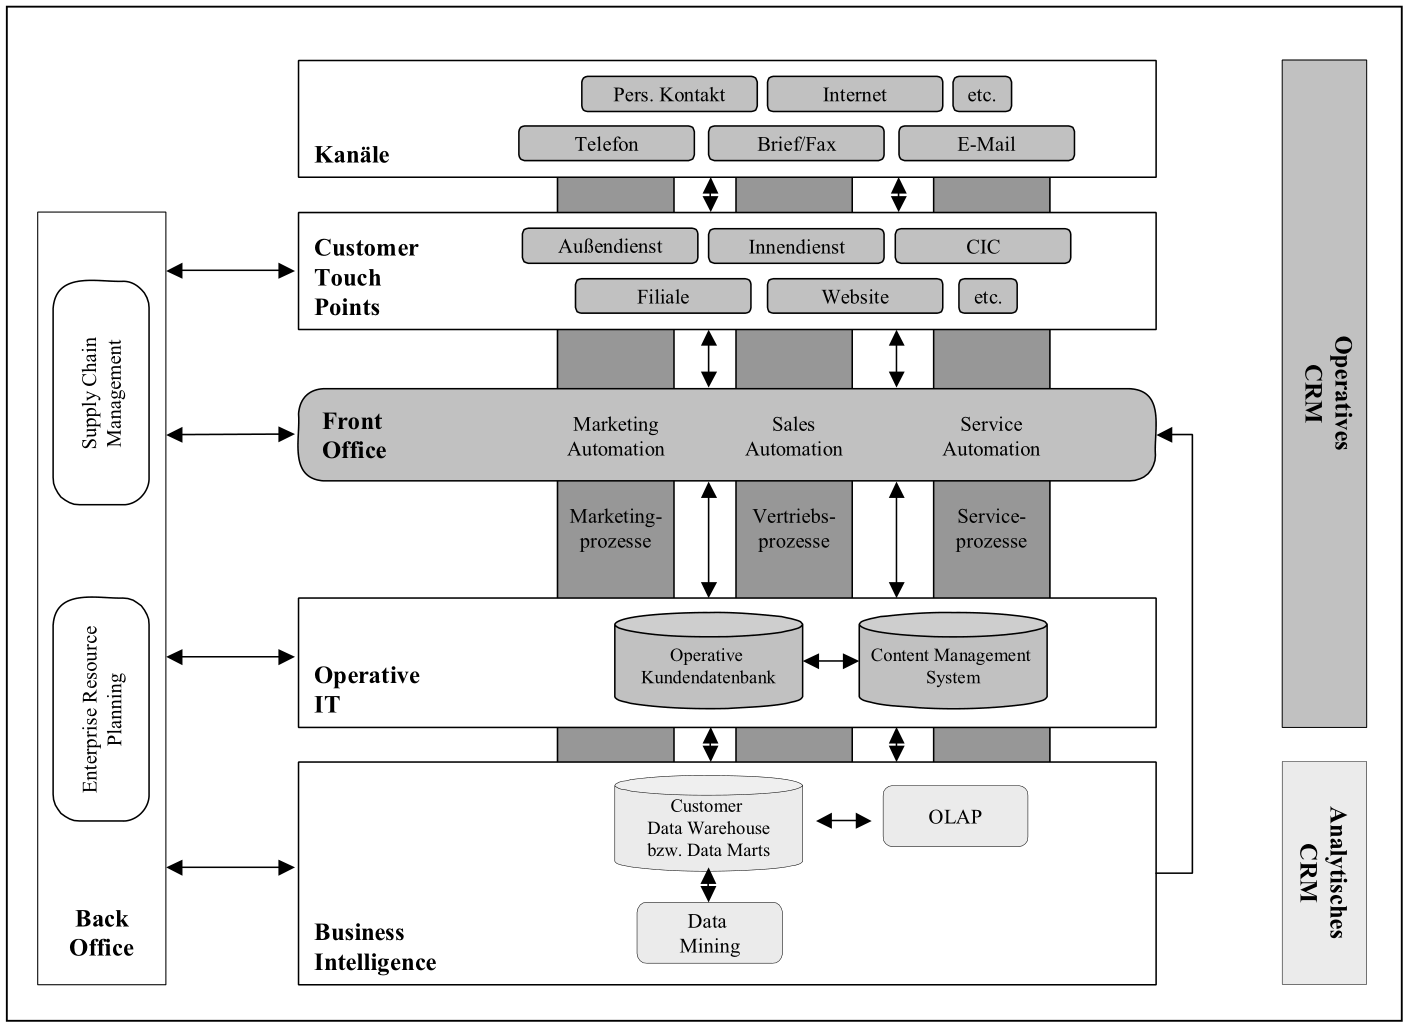
\includegraphics[width=0.9\textwidth]{crmcomps}
  \caption{Komponenten eines CRM-Systems\cite[S. 48]{grundcrm}}
  \label{fig:crmcomps}
\end{figure}

Die für die Business Intelligence relevanten Komponenten lassen sich in OLAP, Data Mining und Customer Data Warehouse bzw. Data Marts einteilen.

\subsection{Data Warehouse und OLAP}

Grundlage für die Differenzierung der Kundenbeziehungen bildet die Zusammenführung aller kundenbezogenen Informationen in einem Customer Data Warehouse, welche eine von der operativen Datenbanken getrennte Analysedatenbank darstellt. \cite[S. 49]{grundcrm}
Man bezeichnet dies auch als Data-Mart, also eine Kopie einer Teilmenge, eines Data Warehouse von in diesem Fall kundenspezifischer Daten. Solche Data-Marts sind üblicherweise hochdimensional und das Finden von in den Daten verborgenen, erfolgsrelevanten Geschäftsinformationen erfordert passende Werkzeuge.
Für diesen Zweck wurde das Konzept des On-Line Analytical Processing (OLAP) entwickelt.
OLAP-Systeme bilden betriebswirtschaftlich relevante Maßgrößen in Form eines multidimensionalen Datenwürfels (Abb. \ref{fig:olap}) ab, dessen Dimensionen betriebswirtschaftlich relevante Gliederungskriterien sind.
Entlang dieser Dimensionen können die betriebswirtschaftlichen Maßzahlen je nach Fragestellung aufgebrochen (Drill down) oder aggregiert (Roll up) werden.
Ergänzend kann der Anwender diesen Würfel drehen und kippen (dice) oder in einzelne \textquote{Scheiben} zerlegen (slice).
\cite[S. 49]{grundcrm}

\begin{figure}[ht]
  \centering
  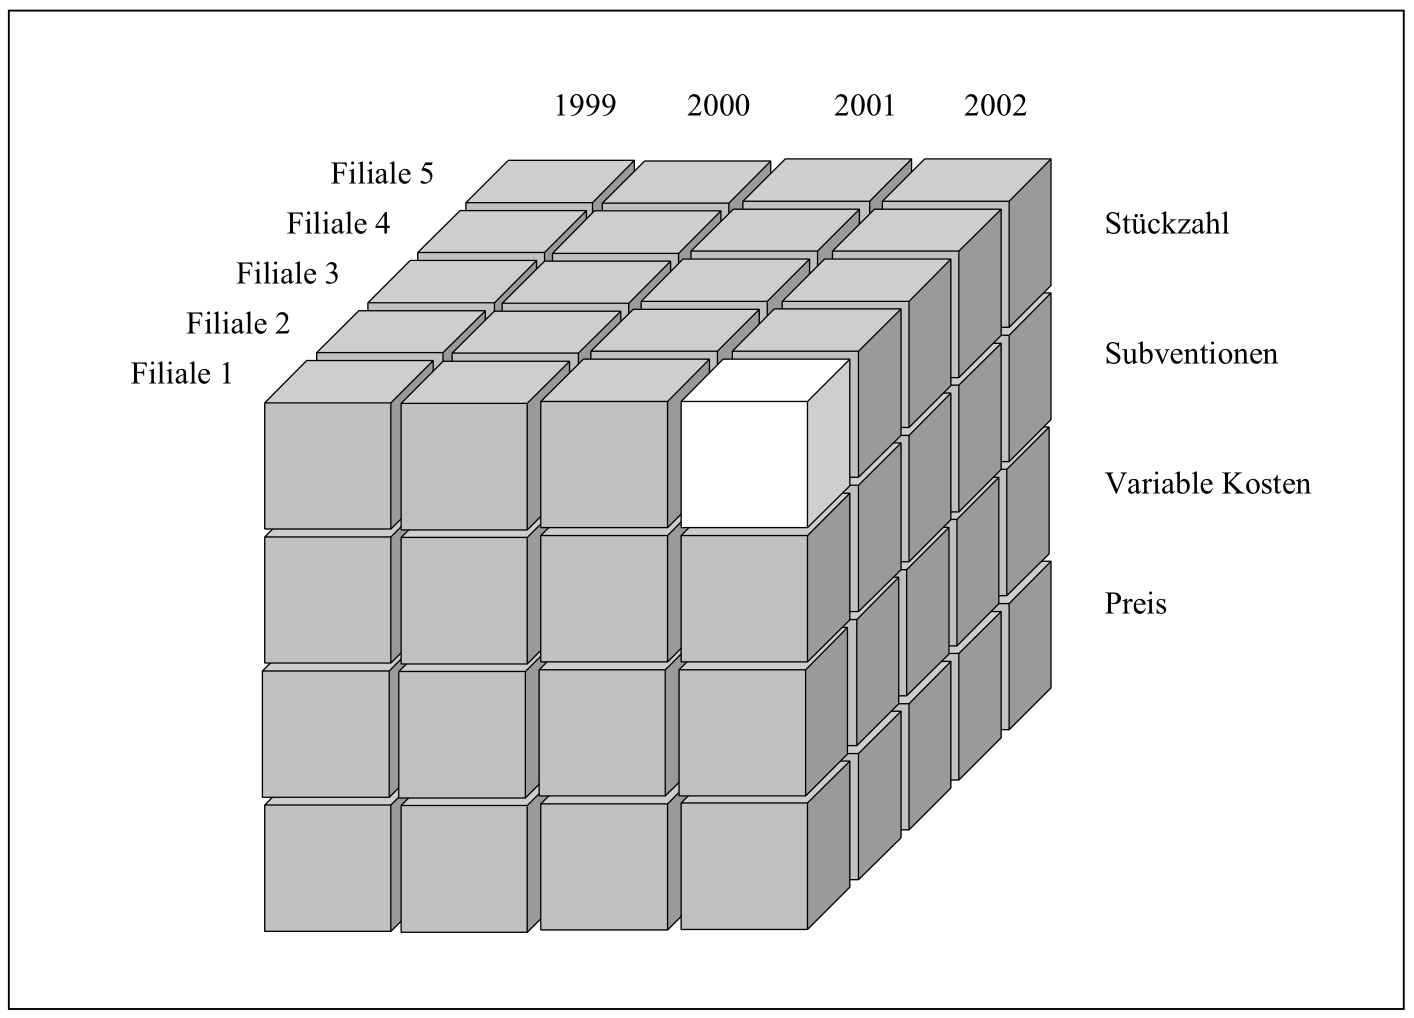
\includegraphics[width=0.9\textwidth]{olap}
  \caption{Beispiel Navigation in einem dreidimensionalen Datenwürfel\cite[S. 50]{grundcrm}}
  \label{fig:olap}
\end{figure}

Zum Erkennen der Zusammenhänge im OLAP-System setzt man Data Mining ein, mit der man die anwenderorientierten Anfragen um automatisierte Suche nach komplexeren Strukturen erweitert.

\subsection{Data Mining Methoden}

Im Rahmen des Data Mining werden Methoden zur Klassifikation, Prognose, Segmentierung und Abhängigkeitsanalyse untersucht und entsprechende Algorithmen entwickelt.

\begin{figure}[ht]
  \centering
  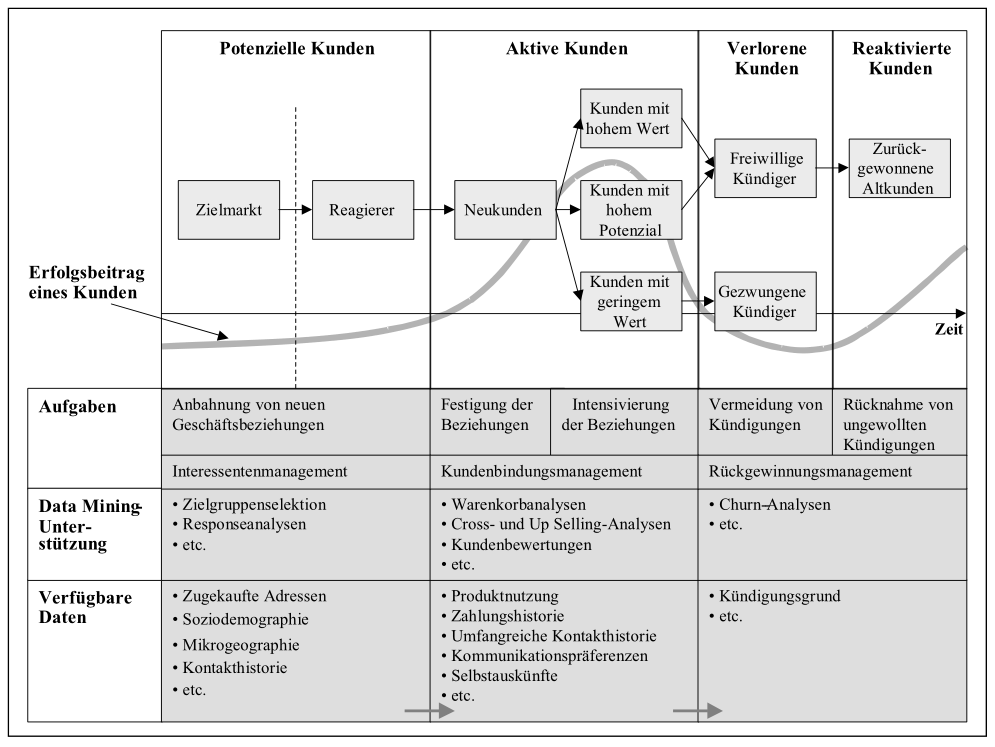
\includegraphics[width=0.9\textwidth]{datamining}
  \caption{Data Mining im Beziehungslebenszyklus\cite[S. 52]{grundcrm}}
  \label{fig:datamining}
\end{figure}

Ein typisches Beispiel der Klassifikation ist die Kündigeranalyse, bei der nach Variablen gesucht wird, die einen möglichst starken Zusammenhang zum Kündigungsverhalten aufweisen und aufgrund derer eine Klassifikation der Kunden möglich wird.
Ein solches Klassifikationsmodell lässt sich auch zur Prognose der Kündigungswahrscheinlichkeit bestehender Kunden einsetzen.
Eine Segmentierung verfolgt das Ziel, Individuen in vorab unbekannte homogene Segmente zusammenzufassen. Hierbei werden durch das Verfahren selbständig Kundensegmente ermittelt, die sich durch ähnliche Merkmalskombinationen auszeichnen.
Ein Beispiel für eine Abhängigkeitsentdeckung ist die Warenkorbanalyse, bei der untersucht wird, welche Produkte typischerweise gemeinsam innerhalb der Käufe eines Kunden auftreten. \cite[S. 51]{grundcrm}

\subsection{Anwendungsbeispiel: CRM im Einzelhandel}

In \cite{biapp} wird ein Beispiel skizziert, in dem ein Unternehmen für eine zielgruppenspezifische Preis- und Rabattpolitik eine Kundenkarte mit einem entsprechenden Bonusprogramm erstellen möchte.

Dazu werden die Verkäufe am Point of Sale (POS) erfasst, in ein Core Data Warehouse geladen und die für die Kampagne relevanten Daten in einem Data Mart zusammengeführt.
Darauf lassen sich dann Analysesysteme für eine Zielgruppenselektion mittels Data Mining Methoden oder klassischen Scorings bzw. o.g. KPIs wie die RFM-Methode \cite{rfmr} aufbauen und für die Zielgruppen die relevantesten Kanäle zum bewerben ermitteln.
Anschließend wird eine Wirkungsanalyse mit dem Ziel der Gewinnung handlungsrelevanter Informationen für den weiteren Verlauf der Kampagne oder zukünfitge Kampagnen durchgeführt. Die Daten aus der Wirkungsanalyse werden dann wieder in den Data Mart eingespeist, um Lernen zu ermöglichen. Dies wird als Closed-loop \cite[S. 223]{biapp} bezeichnet.

Damit erhält man ein Business Intelligence System für die Unterstützung und Steuerung von Entscheidungen, um über CRM den Unternehmenserfolg zu erhöhen. Ein Schema für solch eine Prozesskette ist ist in Abbildung \ref{fig:bieinzel} abgebildet.

Laut \cite[S. 224]{biapp} führte das praktische Umsetzen eines solchen Anwendungsbeispiel zu einer Steigerung der Responsequote um 300\%, während die Anzahl der durchschnittlich angeschriebenen Kunden um 60\% verringert wurde, wodurch das Projekt unternehmensintern als Erfolg gewertet wurde.


\begin{figure}[ht]
  \centering
  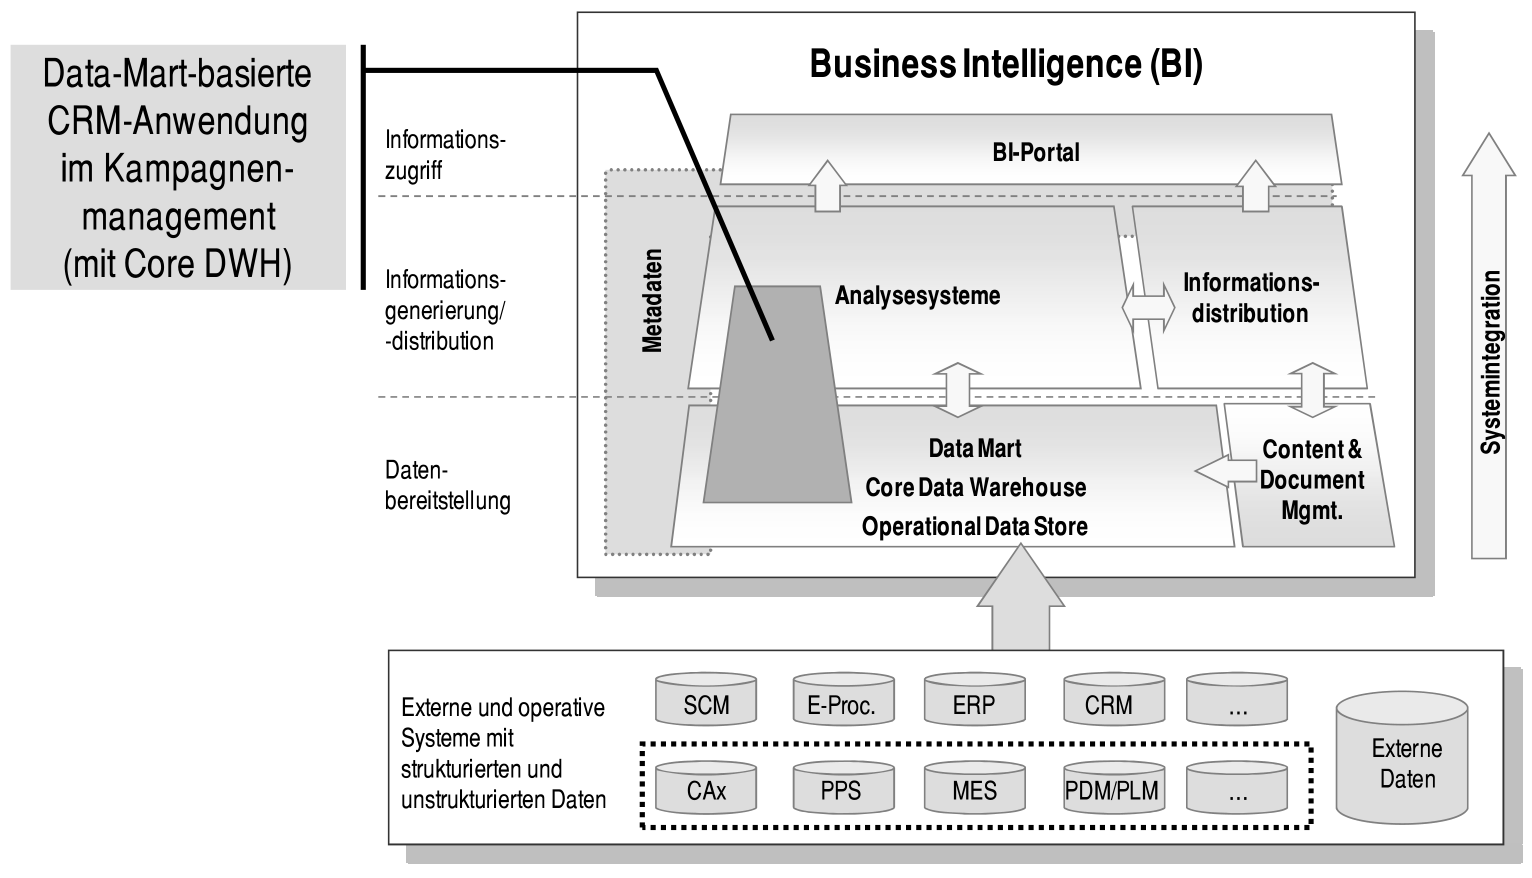
\includegraphics[width=0.9\textwidth]{crmeinzel}
  \caption{CRM im Einzelhandel\cite[S. 220]{biapp}}
  \label{fig:bieinzel}
\end{figure}

\subsection{Anwendungsbeispiel: Supermarket sales (Kaggle)}

In diesem Beispiel wird mögliche Customer Segmentation anhand eines realen Datensatzen aus Kaggle (\url{https://www.kaggle.com/aungpyaeap/supermarket-sales/version/3}) vorgestellt.

Der Datensatz entstammt aus einer Datenerhebung von historischen Verkaufsdaten aus drei Standorten einer Supermarktkette in Myanmar  über drei Monate hinweg.
Jede Zeile ist ein Einkauf und als Feature-Spalten gibt es:

\begin{center}
  \begin{tabular}{l | m{10cm}}
    Invoice id & Computer generated sales slip invoice identification number\\
    Branch & Branch of supercenter (3 branches are available identified by A, B and C).\\
    City & Location of supercenters\\
    Customer type & Type of customers, recorded by Members for customers using member card and Normal for without member card.\\
    Gender & Gender type of customer\\
    Product line & General item categorization groups - Electronic accessories, Fashion accessories, Food and beverages, Health and beauty, Home and lifestyle, Sports and travel\\
    Unit price & Price of each product in \$\\
    Quantity & Number of products purchased by customer\\
    Tax & 5\% tax fee for customer buying\\
    Total & Total price including tax\\
    Date & Date of purchase (Record available from January 2019 to March 2019)\\
    Time & Purchase time (10am to 9pm)\\
    Payment & Payment used by customer for purchase (3 methods are available – Cash, Credit card and Ewallet)\\
    COGS & Cost of goods sold\\
    Gross margin \% & Gross margin percentage\\
    Gross income & Gross income\\
    Rating & Customer stratification rating on their overall shopping experience (On a scale of 1 to 10)
  \end{tabular}
\end{center}

Wie in den Herausforderungen der Customer Analytics aufgezeigt, sind nicht alle erfassten Daten bzw. Features für die Analyse relevant. Daher wurde eine Bereingung vorgenommen.
Für den Anwendungsfall irrelevante Informationen (Steuerbeträge, Gesamtbeträge, Prozentbeträge, Invoice ID) wurden daher im Vorfeld entfernt. Die verbleibenden Daten können dem Schema in Abbildung \ref{fig:fs00} entnommen werden.

\begin{figure}[ht]
  \centering
  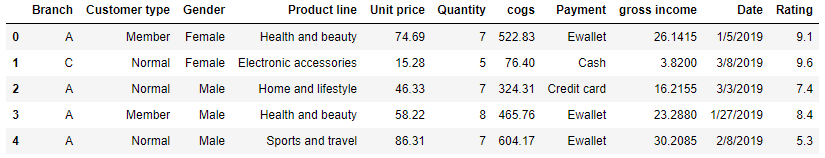
\includegraphics[width=0.9\textwidth]{seg00}
  \caption{Feature Selektion}
  \label{fig:fs00}
\end{figure}

Nach der Bereinigung um irrelevante Features wird, anhand der oftmals aus dem operativen Sektor des CRM stammenden Anfragen, die Grundlage für das Clustering bestimmt.
In diesem Anwendungsbeispiel wird folgende Fragestellung untersucht:

\begin{center}
  \textbf{Gibt es Kundengruppen mit signifikant unterschiedlicher Zufriedenheit?}
\end{center}

Für diese Fragestellung werden die features \textquote{gross income} und \textquote{Date} entfernt, da \textquote{gross income} für den Kunden nicht relevant ist und und \textquote{Date} das Beispiel unnötig Komplex machen würde. Übrig bleibt ein Schema mit Features, auf die der Kunde Einfluss hat (Abb. \ref{fig:fs01}).

\begin{figure}[ht]
  \centering
  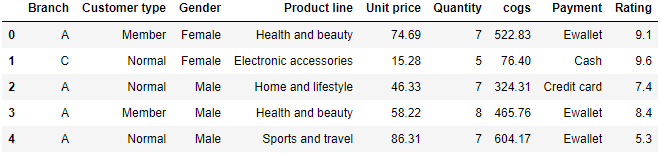
\includegraphics[width=0.9\textwidth]{seg01}
  \caption{Feature Selektion für die Fragestellung}
  \label{fig:fs01}
\end{figure}

Nach der Formulierung der Untersuchungsgrundlage können die Daten weiter um irrelevante Features bereinigt werden.
Daher wird \textquote{gross income} aufgrund fehlender Relevanz entfernt und das Feature \textquote{Date} im Zuge geringerer Komplexität ebenfalls im weiteren Verlauf nicht berücksichtigt.
Damit liegt ein weiter eingegrenztes Schema vor (Abb. \ref{fig:numfeat}).
Unter den Features befinden sich fünf kategorielle Features, von denen zwei binäre Klassen und drei mehrere Klassen besitzen (Abb. \ref{fig:numfeat}).

\begin{figure}[ht]
  \centering
  \begin{tabular}{l | l}
    Feature & Anzahl Ausprägungen\\
    \hline
    Branch & $3$\\
    Customer Type & $2$\\
    Gender & $2$\\
    Product Line & $6$\\
    Payment & $3$
  \end{tabular}
  \caption{Anzahl Ausprägungen in den kategoriellen Features}
  \label{fig:numfeat}
\end{figure}

Für ein Clustering können die kategoriellen Features in numerische Daten transformiert werden.
Durch die anschließende Verwendung eines \textquote{MinMaxScaler} liegt anschließend ein Dataframe gemäß Abbildung \ref{fig:seg02} vor.

\begin{figure}[ht]
  \centering
  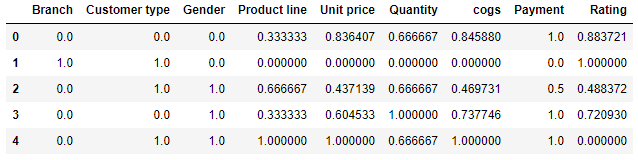
\includegraphics[width=0.9\textwidth]{seg02}
  \caption{Transformierte Daten}
  \label{fig:seg02}
\end{figure}

Für die Wahl der Anzahl an Clustern kann die Elbow-Methode verwendet werden, die auf vier Cluster schließen lässt (Abb. \ref{fig:seg03}).

\begin{figure}[ht]
  \centering
  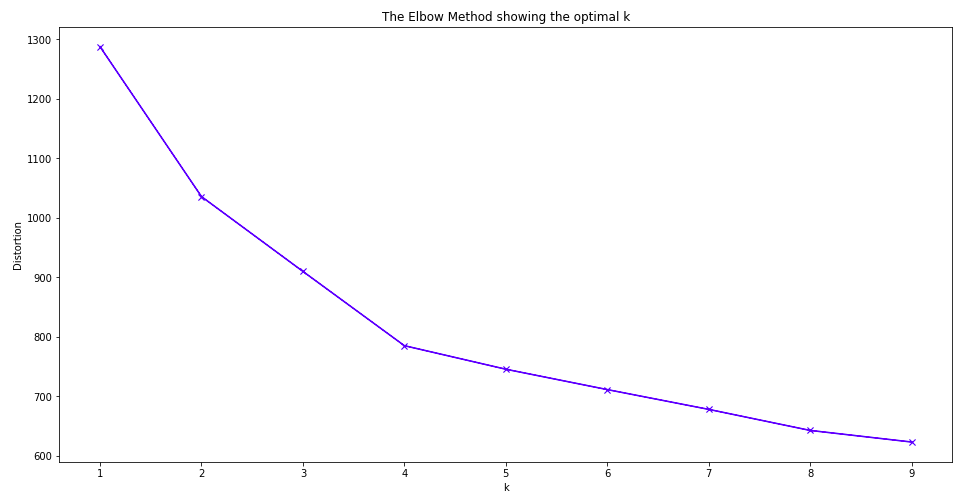
\includegraphics[width=0.9\textwidth]{seg03}
  \caption{Elbow-Methode}
  \label{fig:seg03}
\end{figure}

Aus der Analyse der Ratings innerhalb der Cluster ergeben sich die Zentren aus Abbildung \ref{fig:clusrating}.

\begin{figure}[H]
  \centering
  \begin{tabular}{l | l}
    Cluster & Rating\\
    \hline
    1 & $0.4901021711366539$\\
    2 & $0.5031531531531531$\\
    3 & $0.49$\\
    4 & $0.49840277777777775$
  \end{tabular}
  \caption{Rating Höhe der Cluster}
  \label{fig:clusrating}
\end{figure}

Da die Daten MinMax skaliert sind, bedeutet ein Wert nahe $0.5$, dass der Wert in etwa im Durchschnitt liegt.
Damit kann durch die Auswahl an Features keine Bewertung bezüglich des Ratings abgeleitet werden.

Für die Umsetzung im betrieblichen Kontext bietet es sich an, ein solches Clustering in Business Intelligence Systeme einzubauen, indem man zum Beispiel beliebig Features und Anzahl Cluster auswählen kann und dafür dynamisch den Elbow-Graphen und die Clusterzentren angezeigt bekommt, um so passende Kundensegmentierungen für einzelne Anwendungsfälle der operativen CRM zu erstellen.
